% COMS 6998, Fall 2026 -- final paper working draft.
% Build: latexmk -pdf neural-symbolic-final.tex
\documentclass[conference,10pt,letterpaper]{IEEEtran}
\usepackage[T1]{fontenc}
\usepackage{cite}
\usepackage{amsmath,amssymb}
\usepackage{booktabs,tabularx}
\usepackage{graphicx}
\usepackage{xcolor}
\usepackage{tikz}
\usetikzlibrary{arrows.meta,positioning,fit}
\usepackage{pgfplots}
\pgfplotsset{compat=1.18}
\usepackage[hyphens]{url}
\usepackage[hidelinks]{hyperref}
\newcolumntype{Y}{>{\raggedright\arraybackslash}X}
\newcommand{\draftnote}[1]{\par\smallskip\noindent\textcolor{red!65!black}{\textbf{Draft TODO:} #1}\par\smallskip}
% Generated by generate-results.py; do not edit by hand.
\newcommand{\SerialDeltaAdjusted}{2.506}
\newcommand{\SerialRLAdjusted}{2.502}
\newcommand{\SerialDeltaResidentAdjusted}{2.494}
\newcommand{\SerialRLResidentAdjusted}{2.495}
\newcommand{\DeltaRLDifference}{0.17}
\newcommand{\FaithfulRLSpeedup}{1.55}
\newcommand{\LeanRLSpeedup}{1.20}
\newcommand{\DeltaSat}{10.19}
\newcommand{\DeltaResidentSat}{3.06}
\newcommand{\ResidentReduction}{70.0}


\title{ReasonLink: Characterizing and Optimizing the\\Handoff Between Neural and Symbolic Accelerators}
\author{\IEEEauthorblockN{Vayun Gupta (vg2684), Aaron Mano Cherian (amc2535)}
\IEEEauthorblockA{Columbia University}}

\begin{document}
\maketitle
\thispagestyle{plain}
\pagestyle{plain}

\begin{abstract}
Hardware acceleration reduces computation time within individual pipeline stages, while potentially increasing the fraction of end-to-end execution time attributable to representation conversion, data movement, and synchronization between stages. In neural--symbolic systems, these costs arise when neural outputs are translated into symbolic inputs and exchanged between accelerators. We characterize this interface through visual Sudoku on a VCU118 FPGA system combining NVDLA inference and SAT-Accel reasoning. The full-image baseline repeatedly reconstructs and transfers structural constraints that remain unchanged across puzzles. We introduce ReasonLink, an interface that separates invariant symbolic constraints from input-dependent predictions, enabling compact solver-native updates and reuse of solver state across inputs. Its hardware converts neural outputs into fixed-decision literals, buffers them on chip, and commits them as a compact update; a separate solver modification retains the base formula on chip across inputs. Our evaluation compares full-image preparation, CPU-generated deltas, hardware-generated deltas, on-chip base reuse, and execution overlap, using 100 puzzles per configuration. Preliminary measurements show that the serial full-image baseline, which transfers allocated buffer regions including unused capacity, spends approximately 35\% of its instrumented runtime in the handoff. Compact updates largely eliminate this overhead, and on-chip base reuse reduces median solver time from 10.2 to 3.1\,ms. However, inference dominates the optimized pipeline, and the current measurements do not establish an end-to-end advantage for hardware delta generation over CPU-generated deltas. Within this case study, representation and state reuse capture most of the available performance benefit, while inference limits the additional value of hardware delta generation.
\end{abstract}

\section{Introduction}
Hardware acceleration reduces the cost of computation within individual pipeline stages. End-to-end execution also requires converting the output of one stage into the input representation of the next, transferring that representation, and coordinating execution. These operations can account for a substantial fraction of runtime even when both stages execute on specialized hardware. Understanding their cost is therefore necessary to translate improvements in accelerator performance into improvements in application performance.

Neural--symbolic systems provide a concrete setting for studying this interface. Neural computation produces predictions from unstructured inputs, while symbolic reasoning applies explicit constraints to those predictions. In visual Sudoku, for example, a classifier recognizes handwritten givens and a SAT solver completes the grid. The interface must translate predicted digits into the solver's representation and make them available for reasoning. The Sudoku rules remain unchanged across inputs, yet a full-image host flow reconstructs and transfers the solver's data structures for every puzzle. This repeated preparation couples the cost of supplying new predictions to the size of the shared symbolic representation.

This paper investigates how much of that preparation can be removed through representation and state reuse, and what additional benefit comes from generating updates in hardware. We study an FPGA system built with ESP~\cite{esp}, combining NVDLA for int8 neural inference with SAT-Accel for conflict-driven clause-learning (CDCL) SAT solving~\cite{sataccel}. The system executes perception and reasoning on separate accelerator tiles, providing an end-to-end setting in which to measure conversion, data movement, synchronization, and solver loading.

We introduce ReasonLink, an interface organized around the separation of invariant constraints from input-dependent predictions. The shared rule formula is initialized once, and each new prediction is encoded as a solver-native fixed-decision literal. ReasonLink reads neural outputs, generates and buffers literals in hardware, and writes a compact update to the existing solver image. A complementary on-chip base reuse mechanism retains structural solver data between puzzles and restores the state modified during reasoning. Together, these mechanisms reduce repeated host preparation and internal solver loading.

Our evaluation compares \emph{CPU-generated deltas}, in which CPU software computes literals and writes the update, with \emph{hardware-generated deltas}, in which ReasonLink performs those operations. Both paths use the same fixed-decision representation and support on-chip base reuse. We compare them against full-image preparation and evaluate both sequential execution and execution that overlaps preparation of the next puzzle with the current solve. These configurations evaluate compact updates, computation placement, state reuse, and overlap.

Board measurements show that the handoff accounts for approximately 35\% of instrumented serial runtime when the host rebuilds the solver image and transfers allocated buffer regions, including unused capacity. Compact updates reduce this overhead sharply, while on-chip base reuse reduces median solver time from 10.2 to 3.1\,ms. Neural inference then dominates execution, and CPU-generated and hardware-generated deltas achieve similar end-to-end performance. The resulting characterization identifies both the repeated interface work that can be eliminated and the stage that limits further improvement on this platform.

This paper makes three contributions:
\begin{itemize}
\item An end-to-end characterization of representation conversion, data movement, and synchronization between neural and symbolic accelerators on an FPGA system.
\item ReasonLink, a hardware delta-generation interface, and an on-chip base reuse mechanism that restores solver state across inputs, validated through functional simulation, RTL simulation, and board execution.
\item A comparative evaluation of CPU-generated and hardware-generated deltas, on-chip base reuse, and execution overlap, identifying their effects on interface cost, solver time, and end-to-end performance.
\end{itemize}

\section{Background and Problem Formulation}
\subsection{Neural Perception and SAT Reasoning}
SATNet connects learned perception and satisfiability-based reasoning~\cite{satnet}. Our study instead fixes the trained classifier and solver behavior and varies the systems interface. NVDLA runs a LeNet-style classifier~\cite{lenet,nvdla}; SAT-Accel supplies the CDCL implementation. ESP provides the tiled SoC and third-party accelerator integration~\cite{esp,espnvdla}. We use these components as infrastructure and study the work between inference and solving.

For a cell $(r,c)$ and candidate digit $d\in\{1,\ldots,9\}$, the Boolean variable is
\begin{equation}
v(r,c,d)=81r+9c+d,\qquad r,c\in\{0,\ldots,8\}.
\end{equation}
The extended Sudoku encoding has 729 variables and 11,988 clauses. The shared base formula contains the structural rules. A given contributes a positive literal for the predicted digit. Argmax considers digits 1--9 and resolves ties toward the lowest digit. All compared paths use this same mapping.

SAT-Accel consumes a memory image containing clause storage, clause metadata, literal occurrence lists, mutable clause states, per-variable metadata, and an answer stack. Its host flow already represents unit clauses as level-0 fixed decisions. Consequently, predicted givens can be passed as an answer-stack prefix and a count without rebuilding the structural formula.

\subsection{Measuring the Handoff}
For serial execution, the instrumented stages are
\begin{equation}
T_{\mathrm{inst}}=T_{\mathrm{nn}}+T_{\mathrm{conv}}+T_{\mathrm{xfer}}
                  +T_{\mathrm{sync}}+T_{\mathrm{sat}},
\end{equation}
where conversion includes argmax and image construction, transfer measures the host-side update path, synchronization includes completion handling, and solver time includes internal loading and search. Instrumented stages do not necessarily exhaust process wall time. Their medians also need not sum to a median or mean total.

The serial handoff fraction is computed per puzzle as
\begin{equation}
f_{\mathrm{handoff}}=\frac{T_{\mathrm{conv}}+T_{\mathrm{xfer}}+T_{\mathrm{sync}}}
                              {T_{\mathrm{inst}}},
\end{equation}
and summarized by its median. For double-buffered execution, we record the normalized timing residual
\begin{equation}
R=\frac{T_{\mathrm{wall}}-\sum_i T_{\mathrm{nn},i}-\sum_i T_{\mathrm{sat},i}}
           {T_{\mathrm{wall}}}.
\end{equation}
Overlapping neural and solver execution can make their cumulative durations exceed wall time, yielding $R<0$. The residual reflects both execution overlap and overhead outside the measured stages; end-to-end performance comparisons use wall time.

\subsection{Hypotheses}
We organize the study around two hypotheses:
\begin{itemize}
\item \textbf{H1---Handoff cost:} In serial execution, rebuilding and transferring the full solver image account for a substantial fraction of runtime, dominated by representation preparation rather than the size of the neural outputs.
\item \textbf{H2---Execution overlap:} Double buffering can hide preparation of the next puzzle behind the current solve, but it leaves the amount of representation construction and the transfer volume unchanged. Its benefit depends on the work available to overlap.
\end{itemize}
The board evaluation examines both on visual Sudoku.

% TODO (for later): \draftnote{Add a dedicated related-work section comparing accelerator-interface systems such as DMX and AccelFlow, neurosymbolic architectures, and incremental SAT/state-reuse techniques. Distinguish new mechanisms from those inherited from SAT-Accel and identify the specific contribution beyond existing conversion and reuse mechanisms.}

% TODO (for later): \draftnote{Evaluate a range of workloads beyond Sudoku, including autonomous-driving tasks combining neural perception and symbolic reasoning. For each, define neural outputs, symbolic inputs, reusable constraints, correctness criteria, and the required accelerator support.}

\section{ReasonLink Design}
Figure~\ref{fig:pipeline} shows the shared-memory data paths and control interface.
\begin{figure*}[t]
\centering
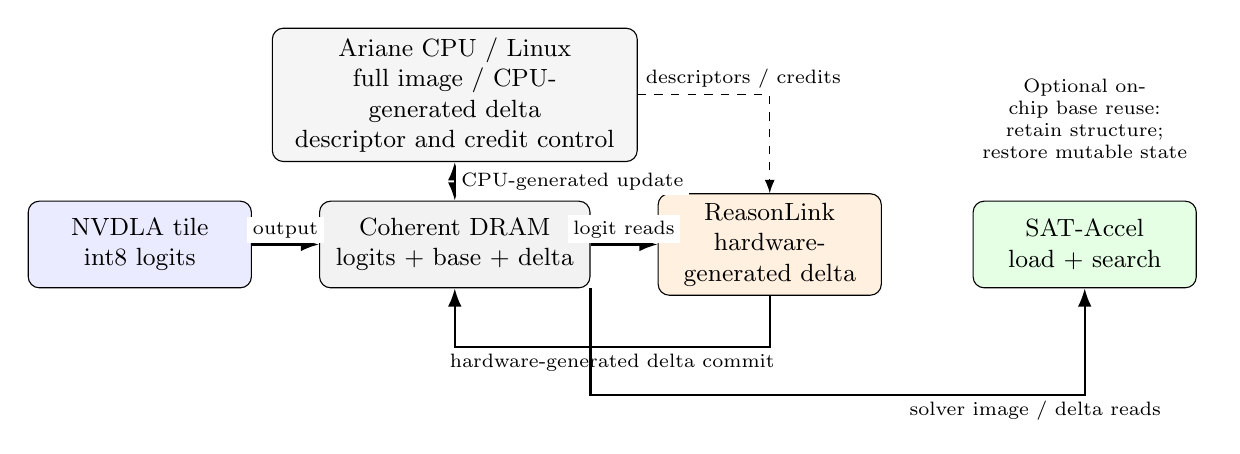
\begin{tikzpicture}[font=\small,>=Latex,
 box/.style={draw,rounded corners,align=center,minimum height=11mm,text width=26mm},
 pathlabel/.style={font=\scriptsize,align=center,fill=white,inner sep=2pt}]
\node[box,fill=blue!8] (nn) at (0,0) {NVDLA tile\\int8 logits};
\node[box,fill=gray!10,text width=32mm] (dram) at (4,0) {Coherent DRAM\\logits + base + delta};
\node[box,fill=orange!12] (rl) at (8,0) {ReasonLink\\hardware-generated delta};
\node[box,fill=green!10] (sat) at (12,0) {SAT-Accel\\load + search};
\node[box,fill=gray!8,text width=44mm] (cpu) at (4,1.9) {Ariane CPU / Linux\\full image / CPU-generated delta\\descriptor and credit control};
\draw[->,thick] (nn) -- node[pathlabel,above]{output} (dram);
\draw[->,thick] (dram) -- node[pathlabel,above]{logit reads} (rl);
\draw[->,thick] (rl.south) -- ++(0,-0.65) -| node[pathlabel,pos=0.25,below]{hardware-generated delta commit} (dram.south);
\draw[->,thick] (dram.south east) -- ++(0,-1.35) -| node[pathlabel,pos=0.45,below]{solver image / delta reads} (sat.south);
\draw[<->,thick] (cpu) -- node[pathlabel,right]{CPU-generated update} (dram);
\draw[->,dashed] (cpu.east) -| node[pathlabel,pos=0.4,above]{descriptors / credits} (rl.north);
\node[font=\scriptsize,align=center,text width=30mm] at (12,1.6) {Optional on-chip base reuse:\\retain structure;\\restore mutable state};
\end{tikzpicture}

\caption{Implemented data paths. NVDLA and SAT-Accel occupy separate ESP tiles. The CPU baseline reads logits and updates a solver image in shared DRAM. ReasonLink receives CPU descriptors, reads logits coherently, queues literals on chip, and commits a compact delta to DRAM. SAT-Accel optionally retains the structural base on chip across solves. Arrows show logical data movement; all cross-tile data traverses the ESP memory system.}
\label{fig:pipeline}
\end{figure*}

\subsection{Compact Fixed Decisions and DRAM Base Reuse}
Both full-image baselines reconstruct the solver representation for every puzzle, including the unchanged structural constraints. The \emph{faithful full-image} baseline follows SAT-Accel's original host-side clearing and transfer policy: it clears capacity-sized clause and literal buffers and transfers allocated image regions, including unused capacity. The \emph{lean full-image} baseline clears previously used clause and literal regions and transfers only the currently used prefixes of the image buffers. On the board, these transfer policies move approximately 5.29\,MB and 632\,KB per puzzle, respectively. The faithful volume is half that of SAT-Accel's default build (10.5\,MB) because clause and literal-store capacities are halved to fit the VCU118 (Section~\ref{sec:impl}). Lean preparation removes unused-capacity overhead but still rebuilds and transfers the complete used representation for every puzzle. Delta updates additionally reuse the existing base image and write only the per-puzzle update.

Both delta paths initialize the base image once and update fixed decisions and counters for each puzzle. In the \emph{CPU-generated delta} path, CPU software reads logits, computes argmax, encodes fixed-decision literals, and writes the update. In the \emph{hardware-generated delta} path (ReasonLink), hardware performs these operations under CPU descriptor control. Both produce equivalent solver inputs, with different transfer layouts. \emph{On-chip base reuse} is a separate solver optimization available to either path. Across the original 1,000-puzzle dataset, only approximately 1,212 bytes of a roughly 632\,KB used image change on average. The implemented CPU-generated delta path moves 3,940 bytes per puzzle, including its update layout and bookkeeping. This is a protocol transfer volume, distinct from the number of semantically changed bytes.

\subsection{Hardware-Generated Delta (ReasonLink)}
ReasonLink resides in the SAT-Accel tile. For each given, software supplies the cell index and the address of NVDLA's output. The core reads ten signed int8 logits from coherent memory, computes argmax over digits 1--9, maps the result to a literal, and queues it in an on-chip FIFO. A commit operation writes the answer-stack delta and relevant counters. The current board path moves 2,948 bytes per puzzle in this commit protocol.

NVDLA reuses an output buffer, so the CPU waits for consumption credit before permitting reuse. This prevents the producer from overwriting logits that ReasonLink has not read. Only the core's conversion of a cell, approximately 85 tile cycles (about 1\,$\mu$s) on the board, can overlap the next inference; descriptor submission and credit polling remain CPU work and cost considerably more (Section~\ref{sec:eval}). The design thus evaluates hardware delta generation behind a shared-memory interface rather than a direct accelerator-to-accelerator wire. The project proposal envisioned a FIFO that bypasses DRAM and a solver that loads state as literals arrive. Because NVDLA and SAT-Accel occupy separate ESP tiles, literals instead reach SAT-Accel through a DRAM commit, and search begins only after the complete delta is committed.

% TODO (for later): \draftnote{Sweep FIFO depth and delta-transfer granularity with fixed predictions and a controlled producer rate. Measure backpressure, CPU descriptor/credit cost, and hardware utilization.}

\subsection{On-Chip Base Reuse and State Restoration}
DRAM base reuse removes host reconstruction but still permits SAT-Accel to reload the same base into on-chip arrays each solve. Resident-base execution additionally retains the base clause store, clause metadata, and literal occurrence storage on chip. A fresh solve populates these arrays; subsequent solves with the same base skip their copy-in.

Correct reuse requires restoring the pre-solve invariant. Base clauses are immutable, but learned clauses can occupy the free tail of each literal's final base page and link to additional pages. Before the next search, the resident path clears those tails and their links. Learned-clause allocators are reinitialized. Mutable clause states, variable metadata, and the answer stack are still copied from DRAM; this implementation does not retain and restore every state structure on chip. Sudoku copy-in falls from roughly 632\,KB to 145\,KB. The tail cleanup is a single line write per literal polarity (1,458 for Sudoku).

The driver enables residency only after a fresh execution with the same base. Back-to-back puzzles must produce the same answers and search counters as independent full-copy executions. Functional probes also compare retained base regions byte for byte after restoration. Merely checking the final Sudoku grid would miss latent learned-state contamination.

% TODO (for later): \draftnote{Add a mechanism-level control/restoration diagram, restoration pseudocode, and state invariants, including learned-clause cleanup, base changes, and buffer reuse. Relate these mechanisms to the incremental-solving techniques discussed in related work.}

\subsection{Execution Overlap}
Serial execution uses one buffer set and completes perception, handoff, and reasoning for puzzle $i$ before starting puzzle $i+1$. Double-buffered execution alternates between two buffer sets: inference, conversion, and transfer for puzzle $i+1$ proceed while SAT-Accel solves puzzle $i$. If that solve is still running when preparation finishes, execution waits for completion before starting the next solve. This scheduling choice is independent of ReasonLink's on-chip literal FIFO, which is used in both execution modes. The solver is not allowed to consume an incompletely committed delta. Base residency remains valid across the two buffers because they represent the same structural formula; retained clause identifiers and on-chip indices do not depend on a particular DRAM buffer address.

\section{Implementation}
\subsection{Platform and Tool Flow}
The prototype is a 2$\times$3 ESP SoC on a VCU118 FPGA, with an Ariane RISC-V processor, NVDLA \texttt{nv\_small}, and a SAT-Accel tile. The nominal tile clock is 78.125\,MHz; per-run counter calibration is approximately 78.1 cycles per microsecond. Linux hosts the application and accelerator drivers. Both accelerator paths use coherent DMA.

The original project proposal named Chipyard and Gemmini. The implemented system uses ESP and NVDLA to match the available integration and tools. SAT-Accel's seven HLS kernels are built with Vitis HLS 2023.2. ReasonLink's hardware delta generator is implemented directly in Verilog RTL; the CPU-generated delta path is software executed by Ariane. On-chip base reuse is implemented in the HLS solver and is available to both delta-generation paths. A custom block design, APB-to-AXI-Lite shell, Linux driver, and user library replace the original \texttt{v++}/XRT integration. Floating-point VSIDS operations remain in the solver, and clause capacity is reduced for the target FPGA.

The resident-base out-of-context SAT-Accel netlist uses 113,062 LUTs; adding ReasonLink increases this to 117,698 LUTs, an incremental 4,636 LUTs (approximately 4.1\%). Both configurations use 434 URAMs, approximately 45.2\% of the device. These are out-of-context synthesized resources, not isolated placed-and-routed overhead. The November 4 rebuilt full-system bitstreams meet timing, with recorded worst setup slack of $+$0.774\,ns for the SAT-Accel build and $+$0.369\,ns for the ReasonLink build.

\draftnote{Archive the final utilization and timing reports alongside exact bitstream and source hashes. Distinguish final routed resources from HLS estimates and out-of-context synthesis in the final resource table. Support any energy-efficiency claims with energy measurements.}

\draftnote{Rebuild the Linux image with the output-layout fix and package the exact executables, bitstreams, source revisions, raw results, and figure-generation scripts used for the final evaluation. Condense the integration bug history to the details needed to explain the design and its validation.}

\subsection{Classifier and Workload}
We retain ESP's LeNet architecture and retrain weights with preprocessing compatible with the int8 runtime. The recorded MNIST test accuracies are 99.17\% in floating point and 99.20\% with the int8 emulator. The board loadable exposes the logits used by the handoff; softmax is unnecessary for argmax.

The generated dataset contains 1,000 unique-solution puzzles with 24--40 clues, with a mean of approximately 32.1. Each given is paired with an MNIST test image. The current board study uses 100 puzzles. Misclassification can make a previously unique puzzle unsatisfiable or introduce alternative solutions, so solver correctness must be assessed against predicted givens, separately from recovery of the original grid.

\subsection{Integration Validation}
Integration exposed failures that component-level tests did not capture. ESP's APB reads could arrive without the setup phase expected by our bridge. ESP's AXI socket also ignored write strobes, allowing result writes to overwrite neighboring bytes; a wrapper adapter corrected the behavior. Full-SoC simulation and a bare-metal board solve validated the resulting path.

On Linux, interrupt acknowledgement and overlapping accelerator DMA reservations caused additional failures. These were corrected before collecting the accepted comparisons. Finally, ReasonLink initially decoded digits 8 and 9 from incorrect channels because the runtime's output stride could not be represented by the selected layout encoding. The driver now uses the supported contiguous layout and rejects unrepresentable strides. Incorrect pre-fix CSVs are preserved for debugging but excluded from the reported result set.

\section{Evaluation}
\subsection{Configurations and Measurement Protocol}
We compare six handoff configurations in serial and double-buffered execution: faithful full image (allocated-region clearing and transfer), lean full image (used-region clearing and transfer), CPU-generated delta, CPU-generated delta + on-chip base reuse, hardware-generated delta (ReasonLink), and hardware-generated delta + on-chip base reuse. A thirteenth configuration replays classifier logits with the faithful serial path. The replay is a diagnostic that removes actual NVDLA execution; it is not a measured faster neural accelerator.

The reported dataset contains one completed 100-puzzle run per configuration. Failed attempts are excluded from these completed-run timings and discussed separately. Model, encoding, predicted digits, and solver settings are held fixed. We report whole-run wall time divided by puzzle count and medians of instrumented per-puzzle stages. The median of a stage and the mean wall time are different statistics and should not be added or subtracted as if they were a single representative execution.

The current wall-time interval excludes initial model, dataset, and base-image loading. Each run has zero warm-up puzzles; the first solve loads on-chip base state even when subsequent solves reuse it. In the hardware-generated path, the inference interval also includes descriptor submission and credit waits. CPU-generated updates are computed after inference for the puzzle, whereas hardware-generated updates can overlap subsequent cell classifications.

\draftnote{Fix the workloads, correctness checks, randomized configuration order, and experiment budget. Repeat clean runs without SSH monitoring; retain raw and summarized data and report uncertainty across independent runs. Specify the warm-up policy and report cold-start costs separately from steady-state performance. Match CPU and hardware update payloads and generation schedules to isolate computation placement, and use consistent timing boundaries for conversion, submission, transfer, and synchronization.}

Some runs included SSH monitoring that competed for the board's slow CPU. The existing summarizer estimates excess inference time using each run's median inference time per given. For puzzle $i$, with $g_i$ givens, it computes
\begin{align}
b &= \operatorname{median}_i(T_{\mathrm{nn},i}/g_i),\\
\widehat{S} &= \sum_i\max(T_{\mathrm{nn},i}-b g_i,0),\\
\widehat{T}_{\mathrm{wall}} &= T_{\mathrm{wall}}-\widehat{S}.
\end{align}
This adjustment attributes all above-median inference excess to interference and may remove real variation as well. We show it as an estimate alongside measured wall time. It does not replace clean repeats or support statistical significance. A later five-configuration double-buffered batch ran without SSH monitoring and completed 500 puzzles without a hang; independent repeated batches are still needed.

\draftnote{Use clean repeated measurements for final headline comparisons. Separate NVDLA device time from runtime/driver overhead, and measure sensitivity to neural production rate, solver difficulty, and symbolic-state size. Compare against the optimized CPU-generated delta path as well as full-image baselines. Add a figure showing the measured regimes where CPU-generated deltas, hardware-generated deltas, and on-chip base reuse are beneficial.}

\begin{figure*}[t]
\centering
\begin{tikzpicture}
\begin{axis}[name=serial,width=0.49\textwidth,height=5.2cm,
 ybar,bar width=7pt,ymin=0,ymax=4.6,
 ylabel={Seconds per puzzle},title={Serial},
 xtick=data,xticklabels={Faithful,Lean,CPU delta,CPU delta+B,HW delta,HW delta+B},
 x tick label style={font=\scriptsize,rotate=25,anchor=east},
 enlarge x limits=0.12,grid=major,grid style={gray!15},
 legend style={font=\scriptsize,at={(0.98,0.98)},anchor=north east,legend columns=1},
 tick label style={font=\scriptsize}]
\addplot[fill=blue!55,draw=blue!70] table[x=index,y=measured_s,col sep=tab]{figures/serial-walltime.tsv};
\addplot[fill=orange!65,draw=orange!80!black] table[x=index,y=adjusted_s,col sep=tab]{figures/serial-walltime.tsv};
\legend{Measured,Adjusted estimate}
\end{axis}
\begin{axis}[at={(serial.east)},anchor=west,xshift=0.6cm,
 width=0.49\textwidth,height=5.2cm,ybar,bar width=7pt,ymin=0,ymax=4.6,
 title={Double-buffered},
 xtick=data,xticklabels={Faithful,Lean,CPU delta,CPU delta+B,HW delta,HW delta+B},
 x tick label style={font=\scriptsize,rotate=25,anchor=east},
 enlarge x limits=0.12,grid=major,grid style={gray!15},
 tick label style={font=\scriptsize}]
\addplot[fill=blue!55,draw=blue!70] table[x=index,y=measured_s,col sep=tab]{figures/double-walltime.tsv};
\addplot[fill=orange!65,draw=orange!80!black] table[x=index,y=adjusted_s,col sep=tab]{figures/double-walltime.tsv};
\end{axis}
\end{tikzpicture}

\caption{Mean wall seconds per puzzle from the current 100-puzzle board runs. Measured wall times and the repository's interference-adjusted estimates are shown separately. Each bar represents one completed run; no error bars or significance claims are available. CPU delta and HW delta denote CPU-generated delta and hardware-generated delta (ReasonLink); +B enables on-chip base reuse for either path.}
\label{fig:wall}
\end{figure*}

\subsection{H1: Full-Image Preparation Is Substantial}
Table~\ref{tab:serial} reports serial-stage medians. The faithful baseline spends approximately 722\,ms building its image and 609\,ms in transfer, compared with approximately 11\,ms in SAT-Accel loading and search. Its median instrumented handoff fraction is 34.9\%. Lean clearing and transfer reduce these stages to approximately 412 and 73\,ms, respectively, but preparation remains visible at a 16.3\% handoff fraction.

CPU-generated deltas reduce conversion and transfer to approximately 0.148 and 0.336\,ms. The CPU-generated delta path's median handoff fraction is 0.042\%; the hardware-generated delta path's recorded fraction is approximately 0.024\%. ReasonLink descriptor pushes and credit waits occur inside the inference interval, so this fraction is not a complete hardware-interface cost. Separate diagnostic timing records approximately 18\,$\mu$s of CPU push and credit work per given, or about 0.6\,ms per puzzle.

Host-side transfer volume falls from 5,293,556 bytes in the faithful path and 632,436 bytes in the lean path to 3,940 bytes for CPU-generated delta and 2,948 bytes for hardware-generated delta. These counts exclude NVDLA traffic and SAT-Accel's internal copy-in reads. They therefore quantify the handoff update protocol, not total system memory traffic.

\begin{table*}[t]
\centering
\caption{Serial board-stage medians in milliseconds per puzzle. Base reuse denotes on-chip base reuse; hardware-generated delta is ReasonLink. Host update bytes are distinct from internal solver loads. ReasonLink submission and credit handling are included in $T_{\mathrm{nn}}$; zero CPU conversion does not imply zero interface work.}
\label{tab:serial}
\small
\begin{tabular}{@{}lcrrrrrr@{}}
\toprule
Delta generation / baseline & Base reuse & $T_{\mathrm{nn}}$ & $T_{\mathrm{conv}}$ & $T_{\mathrm{xfer}}$ & $T_{\mathrm{sync}}$ & $T_{\mathrm{sat}}$ & Update bytes\\
\midrule
Faithful full image & No & 2537.826 & 721.970 & 609.000 & 0.723 & 10.995 & 5,293,556 \\
Lean full image & No & 2530.492 & 411.617 & 73.198 & 0.551 & 10.645 & 632,436 \\
CPU-generated delta & No & 2547.761 & 0.148 & 0.336 & 0.563 & 10.192 & 3,940 \\
CPU-generated delta & Yes & 2458.728 & 0.147 & 0.336 & 0.545 & 3.058 & 3,940 \\
Hardware-generated delta & No & 2618.511 & 0.000 & 0.060 & 0.552 & 10.118 & 2,948 \\
Hardware-generated delta & Yes & 2615.484 & 0.000 & 0.060 & 0.538 & 3.005 & 2,948 \\
\bottomrule

\end{tabular}
\end{table*}

\subsection{CPU-Generated Versus Hardware-Generated Deltas}
Figure~\ref{fig:wall} shows that the optimized paths cluster near 2.5\,s per puzzle after adjustment. CPU-generated delta takes \SerialDeltaAdjusted\,s per puzzle and hardware-generated delta takes \SerialRLAdjusted\,s, a difference of only \DeltaRLDifference\% in the adjusted estimates. With on-chip base reuse, the corresponding values are \SerialDeltaResidentAdjusted\,s and \SerialRLResidentAdjusted\,s. Given the unequal monitoring interference and absence of independent repeats, these differences do not establish a hardware speedup.

Relative to faithful serial execution, ReasonLink's adjusted comparison is approximately \FaithfulRLSpeedup$\times$; relative to lean serial execution it is approximately \LeanRLSpeedup$\times$. These gains combine the representation change and execution mechanisms. The CPU-generated delta result shows that base reuse and compact updates already capture almost all of the available end-to-end benefit in the current platform.

\subsection{On-Chip Base Reuse Reduces Solver Loading}
Enabling residency in the CPU-generated delta path reduces median serial SAT time from \DeltaSat\,ms to \DeltaResidentSat\,ms, approximately \ResidentReduction\%. The hardware-generated delta path shows a similar change, from approximately 10.1 to 3.0\,ms. This stage improvement has little effect on the approximately 2.5-second pipeline because inference dominates.

RTL sequences provide separate evidence for the mechanism. After a common fresh first solve, resident puzzle 3 takes 100,553 busy cycles versus 207,383 with full copy-in; resident puzzle 5 takes 81,549 versus 188,379. Read beats fall from approximately 81,400 to 20,800. These are testbench results with a 30-cycle read latency and one outstanding burst, rather than predictions of board runtime. They establish reduced loading under that memory model, with unchanged answers and search counts.

\subsection{H2: Overlap Does Not Remove Repeated Preparation}
Faithful double buffering measures approximately 3.944\,s per puzzle, versus 3.978\,s serial; lean double buffering measures 2.962\,s versus 3.037\,s serial. The current overlap arrangement therefore leaves substantial preparation exposed for full-image paths. It does not reduce the host update bytes.

CPU-generated and hardware-generated delta double-buffered runs measure approximately 2.47\,s per puzzle. Differences from serial include overlap, unequal interference, and a roughly 1\% change in observed per-cell neural time in the later batch. The present data cannot attribute all throughput differences to double buffering. The optimized paths yield slightly negative $R$, consistent with overlap between solver and neural execution.

\subsection{Correctness and Boundary Cases}
All 13 accepted configurations agree on SAT/UNSAT and grids for all 100 board puzzles. The summarizer reports 98 reference-equivalent cases and two valid alternative grids per configuration. Its reference-equivalent category includes matching UNSAT outcomes; the 98 count is not a count of 98 identical solved grids. Alternative grids satisfy Sudoku constraints and retain every predicted given. These checks establish interface equivalence, not 100\% recovery of ground-truth puzzles. Across the full 1,000-puzzle emulated workload, the recorded ground-truth puzzle accuracy is 79.0\%.

Functional resident-state validation covers 1,000 Sudoku puzzles and 192 fixed-decision benchmark instances. Resident and fresh executions agree on models and search counters, and the restored base regions match byte for byte. Without tail cleanup, stale literal-store bytes remain in some instances, demonstrating why explicit restoration is needed.

NVDLA and the emulator differ in the logits of 925--926 given-cell classifications per board run, but the selected digits agree on the evaluated 100 puzzles. Logit-level bit equivalence has therefore not been established for the retrained board model. Two earlier NVDLA mid-task hangs also required FPGA reprogramming; their trigger is unresolved. The later uninterrupted batch is evidence of a successful run, not proof that the reliability issue has been eliminated.

\draftnote{Quantify logit differences, measure ground-truth board accuracy separately, and report failed-attempt frequency and timeout policy. Add a controlled failure/boundary study beyond these observed integration cases.}

\section{Discussion and Remaining Evaluation}
\label{sec:discussion}
\subsection{Where the Benefit Comes From}
The primary observed benefit is eliminating repeated construction and movement of a shared formula. Hardware argmax is one way to produce the resulting small update, but the optimized CPU path also produces it cheaply. Once both paths reduce interface work to approximately a millisecond per puzzle, Linux-managed NVDLA execution dominates the approximately 2.5-second pipeline. Increasing conversion throughput alone has little remaining end-to-end opportunity in this setting.

The optimized system is therefore not yet a balanced producer--consumer pipeline. Each given is a separate NVDLA inference submitted through Linux, at approximately 79\,ms per cell, or about 2.49\,s for 31.4 givens; the producer is roughly 250--800 times slower than a 3--10\,ms solve and accounts for about 99\% of a delta run. LeNet on \texttt{nv\_small} should require far less time, so most of this interval is likely spent in NVDLA's user-mode runtime and kernel driver on the 78\,MHz Ariane core, although we have not separated device time from software time. The CPU also mediates every cell: it submits the inference, waits for completion, pushes a ReasonLink descriptor, and polls for the credit before reusing NVDLA's single output buffer.

This result depends on the deployment. Classifying all givens of a puzzle in one NVDLA submission would reduce $T_{\mathrm{nn}}$ substantially and allow one ReasonLink push per puzzle instead of one per cell; multiple output buffers would let NVDLA run ahead of the SAT-Accel tile. Under either change, conversion and submission costs that are currently hidden would become visible, and the comparison between CPU-generated and hardware-generated deltas could change. The replay diagnostic marks the opposite extreme: with inference removed, the faithful handoff is 99.2\% of instrumented runtime, but a full-image replay alone does not show where the two delta paths diverge. More expensive SAT search would instead amortize both neural and handoff work. Passing non-Sudoku functional checks does not constitute a performance study on harder workloads.

\subsection{Limits of the Current Evidence}
The evaluation uses one small structured workload family and 100 board puzzles per completed configuration. Sudoku is largely propagation dominated, so it is particularly suited to revealing loading and initialization overhead. Capacity limits, large learned-clause populations, sustained buffer backpressure, and long-running searches remain insufficiently explored. No power or energy measurements are available. Synthesized LUT comparisons are useful implementation context, but the current prototype does not establish an energy or area-efficiency advantage.

Measurement interference is another material limitation. A model-based subtraction can help diagnose the board's behavior, but raw timings and clean repeated runs must carry the final claims. The control path also retains per-cell CPU submissions and a DRAM round trip, so these results do not evaluate a fully autonomous direct-stream design.

\section{Conclusion}
ReasonLink separates invariant symbolic constraints from input-dependent predictions in an FPGA neural--symbolic pipeline. Compact fixed-decision updates reduce repeated host preparation and transfer, while on-chip base reuse reduces solver loading. On the evaluated ESP/NVDLA/SAT-Accel system, CPU-generated and hardware-generated deltas achieve similar end-to-end performance after these optimizations, with neural inference dominating the remaining runtime. The characterization identifies representation and state reuse as the principal sources of improvement in this workload.

% TODO (for later): \draftnote{Incorporate responses to midterm and milestone feedback and record individual contributions in the final course submission. Update the abstract, introduction, and conclusion to reflect the completed evaluation, replacing provisional and future-tense statements with established findings. Consolidate measurement qualifications in the methodology and focus the discussion on the mechanisms and conditions explaining the results.}


\bibliographystyle{IEEEtran}
\bibliography{neural-symbolic-references,p1-additional-references}
\appendices
\input{sections/appendix}
\end{document}
